
%%%% Encodings

\usepackage[utf8]{inputenc} % encoding
\usepackage[english]{babel} % use special characters and also translates some elements within the document.

\usepackage{parskip}        % \par starts on left (not idented)

\usepackage[numbers]{natbib} % \citet et al
\usepackage[nottoc]{tocbibind} % Adds the bibliography to the table of contents.

% Hyperlinks \url{url} or \href{url}{name}
\usepackage[colorlinks = true,
            linkcolor = blue,
            urlcolor  = blue,
            citecolor = blue,
            anchorcolor = blue]{hyperref}


% \usepackage[document]{ragged2e}  % Left-aligned (whole document)
% \begin{...} ... \end{...}   flushleft, flushright, center

%%%% Abstract

\usepackage{abstract} % Abstract

% http://www.ctex.org/documents/packages/special/abstract.pdf
\renewcommand{\absnamepos}{flushleft} % \begin{abstract} \noindent ... \end{abstract}
\setlength{\absleftindent}{0pt}
\setlength{\absrightindent}{0pt}

%%%% Math

% Some packages depend on amsmath like semantic

\usepackage{amsmath}
\usepackage{amssymb} % \mathbb{N}
\usepackage{bm} % $\bm{D + C}$

% \begin{theorem}\label{t:label}  ...  \end{theorem}
% \begin{proof} ... \end{proof}
\usepackage{amsthm} % \newtheorem, \proof, etc
\theoremstyle{plain} % default
\newtheorem{theorem}{Theorem}[section]
\newtheorem{corollary}{Corollary}[theorem]
\newtheorem{lemma}[theorem]{Lemma}
\theoremstyle{definition}
\newtheorem{definition}{Definition}[section]
\theoremstyle{remark}
\newtheorem*{remark}{Remark}

% Defines a new environment to write your or claim - proof
\newenvironment{claim}[1]{\par\noindent\underline{Claim:}\space#1}{}
\newenvironment{claimproof}[1]{\par\noindent\underline{Proof:}\space#1}{\hfill $\blacksquare$}

%%%% Graphics

\usepackage{graphicx}
\graphicspath{{./figures/}}

% \begin{figure}[h]
%   \centering
%   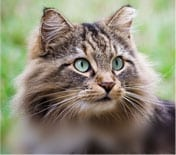
\includegraphics[scale=0.5]{cat}  % [width=\textwidth, height=4cm],
%   \caption{Example of a cat}
%   \label{fig:cat}
% \end{figure}

%%%% Graphs

% Use python instead: https://graphviz.readthedocs.io/en/stable/

% \usepackage{tikz} % https://texample.net/tikz/examples/tag/graphs/

% \begin{tikzpicture}
% \def \n {5}
% \def \radius {3cm}
% \def \margin {8} % margin in angles, depends on the radius

% \foreach \s in {1,...,\n}
% {
%   \node[draw, circle] at ({360/\n * (\s - 1)}:\radius) {$\s$};
%   \draw[->, >=latex] ({360/\n * (\s - 1)+\margin}:\radius)
%     arc ({360/\n * (\s - 1)+\margin}:{360/\n * (\s)-\margin}:\radius);
% }
% \end{tikzpicture}

%%%% Flag derivation

% https://osl.ugr.es/CTAN/macros/latex/contrib/flagderiv/flagderiv.pdf
\usepackage{flagderiv}

% \begin{flagderiv}
%   \introduce{in-x}{x: \mathbb{N}}{Introduction of $x$}
%     \assume{as-x}{x > 5}{Assumption}
%       \step{big-x}{x > 1}{Arithmetic on \ref{in-x} and \ref{as-x}}
%     \conclude{conc}{x > 5 \implies x > 1}{$\implies$-intro on \ref{as-x} and \ref{big-x}}
%   \conclude{}{\forall x \in \mathbb{N} : x > 5 \implies x > 1}{$\forall$-intro on \ref{in-x} and \ref{conc}}
% \end{flagderiv}

%%%% Semantic: inference, tdiagram, shorthands

% https://osl.ugr.es/CTAN/macros/latex/contrib/semantic/semantic.pdf
\usepackage{semantic} % depends on amsmath

% \mathlig{-><-}{\rightarrow\leftarrow}
% $-><-$ \mathligsoff $-><-$ \mathligson $-><-$

% The following ligatures are provided:
% |-   |=
% <->  <=>
% ->   -->
% =>   ==>
% <-   <--
% <=   <==
% ->*  ->+   ==>* ...

% \inference[$->*_{1}$]{
%   \inference[$->*_{2}$]{
%     \inference[$->*_{3}$]{
%       \rho |- E => TRUE
%     }{\rho \vdash E do s}
%   }{\rho \vdash E do s}
%   &
%   \inference[$->*_{2}$]{
%     \rho |- E => TRUE
%   }{\rho \vdash E do s}
% }{\rho \vdash E do s}

% denotational semantics are also supported (see docs)

%%%% Tables
\usepackage{booktabs} % better default table

% \begin{table}
% \centering
% \caption{This is my table, there are many like it, but this one is mine.}
% \label{tbl:mytable}
% \begin{tabular}{llr}
% \toprule
% \multicolumn{2}{c}{Item} \\
% \cmidrule(r){1-2}
% Animal & Description & Price (\$) \\
% \midrule
% Gnat  & per gram & 13.65 \\
%       & each     &  0.01 \\
% Gnu   & stuffed  & 92.50 \\
% Emu   & stuffed  & 33.33 \\
% Armadillo & frozen & 8.99 \\
% \bottomrule
% \end{tabular}
% \end{table}

%%%% Code/Pseudo-code

\usepackage{minted} % Code listing
% \mint{html}|<h2>Something <b>here</b></h2>|
% \inputminted{octave}{BitXorMatrix.m}

%\begin{listing}[H]
  %\begin{minted}[xleftmargin=20pt,linenos,bgcolor=codegray]{haskell}
  %\end{minted}
  %\caption{Example of a listing.}
  %\label{lst:example} % You can reference it by \ref{lst:example}
%\end{listing}

\newcommand{\code}[1]{\texttt{#1}} % \code{foo.hs} environment

\usepackage[vlined,ruled]{algorithm2e} % pseudo-code

%%%% Colors

\usepackage{xcolor} % \definecolor, \color{codegray}
\definecolor{codegray}{rgb}{0.9, 0.9, 0.9}
% \color{codegray} ... ...
% \textcolor{red}{easily}

%%%% Glossaries

%\makeglossaries % before entries

%\newglossaryentry{latex}{
    %name=latex,
    %description={Is a mark up language specially suited
    %for scientific documents}
%}

% Referencing a glossary \gls{latex}
% Print glossaries \printglossaries


%%%% Acronyms

\usepackage[acronym]{glossaries} %

% \acrshort{name}
% \acrfull{name}
% \newacronym{foo}{arcshort}{acrfull}


%%%% Better enumerate

\usepackage{enumitem} % \begin{enumerate}[label=(\alph*)]
